%\begin{figure*}[tbh]
%	\centering
%	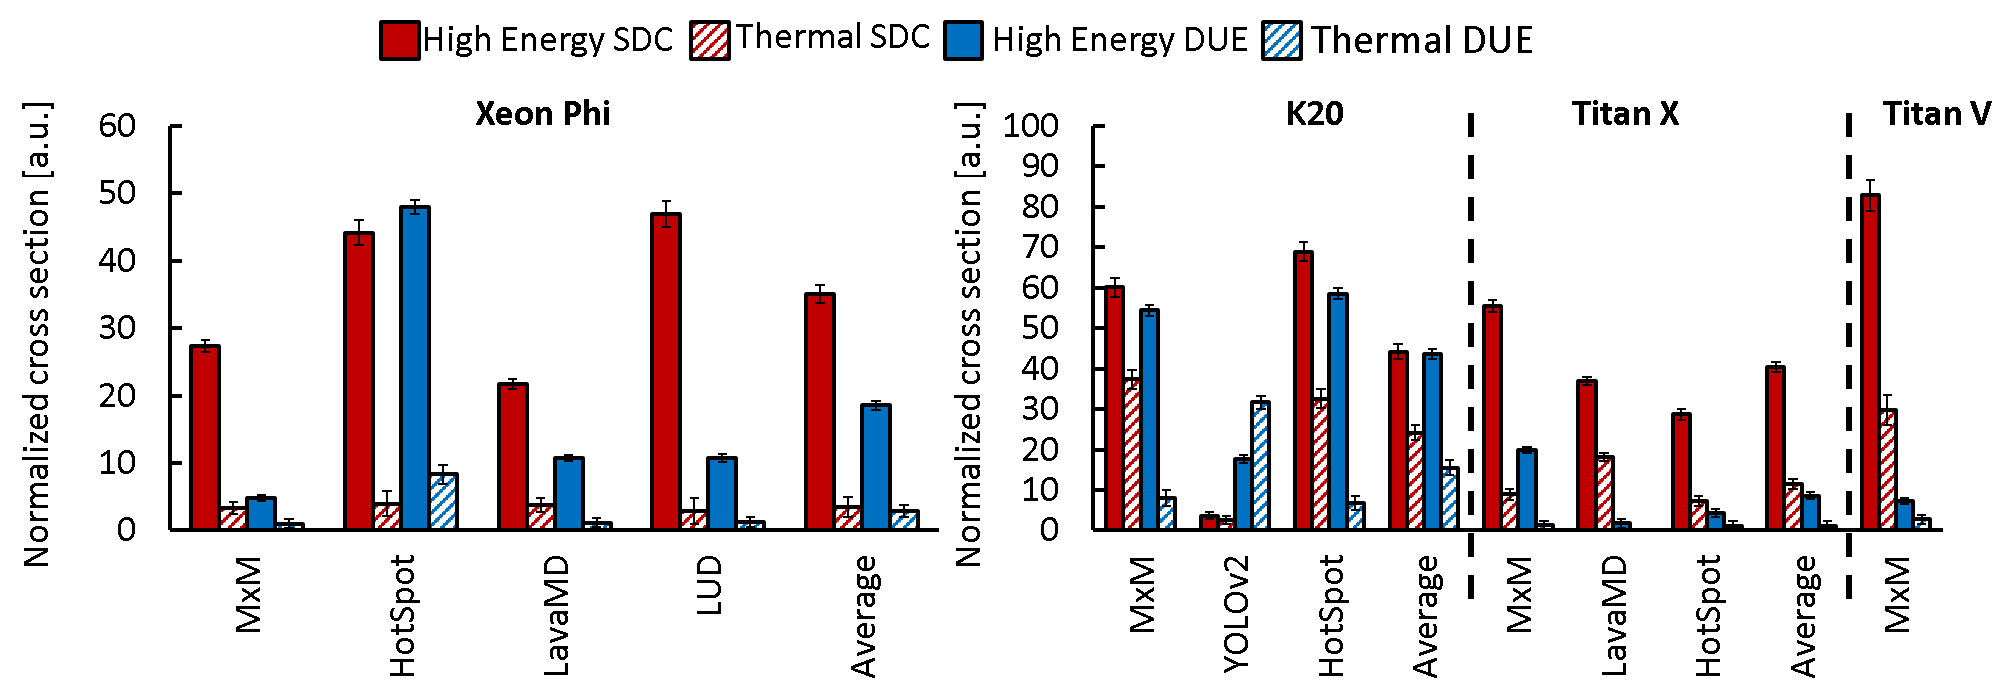
\includegraphics[width=0.81\textwidth]{./data/plots_final/cs_xeon_gpus_avg.png}
%	\caption{High energy and thermal neutrons normalized cross sections for Xeon Phi and GPUs.}
%	\label{cs_xeon_gpus}
%\end{figure*}
%
%\begin{figure*}[th]
%	\centering
%	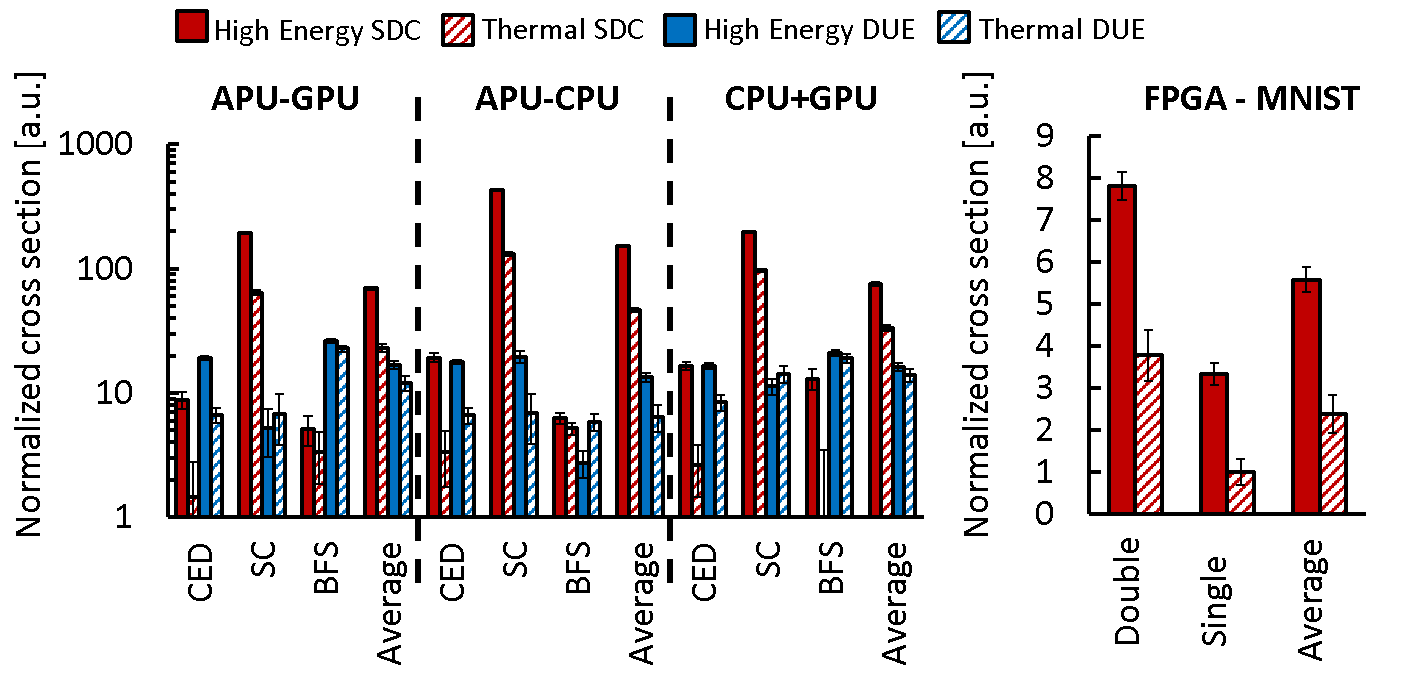
\includegraphics[width=0.75\textwidth]{./data/plots_final/cs_APU_FPGA_avg.png}
%	\caption{High energy and thermal neutrons normalized cross sections for AMD APU and FPGA.}
%	\label{cs_apu_fpga}
%\end{figure*}

\begin{figure*}[th]
	\centering
	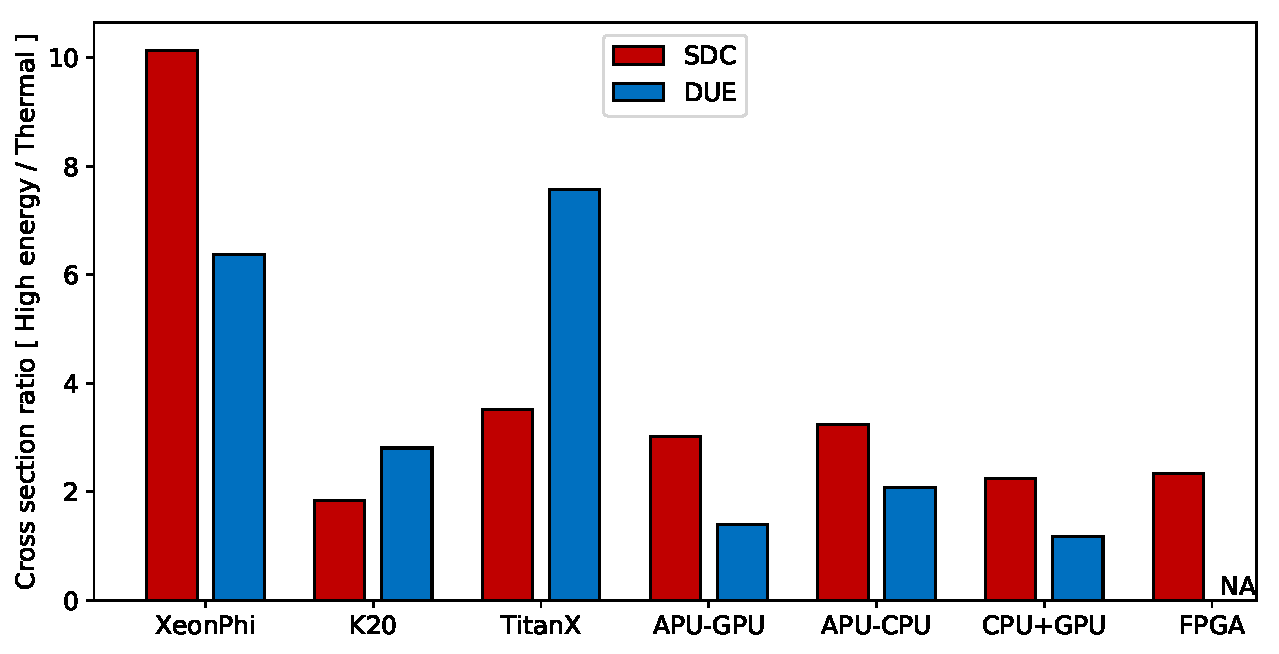
\includegraphics[width=0.85\textwidth]{./figs/cross_section_ratio.pdf}
	\caption{Average cross section ratio for all devices.}
	\label{cs_ratio}
\end{figure*}

\section{Cross Section Results}
\label{sec_results}

In this section, we show the average cross sections results from ChipIR and ROTAX experiments. It is important to note that we used the same device and setup for both experiments. As we show, the thermal neutrons cross section is far from being negligible, which indicates the presence of $^{10}B$ in the silicon doping.

Figure~\ref{cs_ratio} compares the sensitivity of high energy and thermal neutron cross sections. We divide the high energy cross section by the thermal neutron one, to provide the ratio between the cross sections. In other words, a cross section ratio close to one implies that the thermal neutron cross section is highly significant.

For \textbf{Xeon Phi}, the ratio is 10.14x for SDCs and 6.37x for DUEs as shown in Figure~\ref{cs_ratio}. Thus, for each SDC caused by thermal neutrons, we have about 10 SDCs caused by high energy ones. This low sensitivity to thermal neutrons indicates that Xeon Phi uses little or depleted boron in the manufacturing of the devices.

\textbf{NVIDIA GPUs} SDC ratio is about 2x to 3x for K20 and TitanX, respectively. For DUE, the difference is even more substantial,  with K20 presenting a ration of 3x while TitanX has a ratio of 7x. TitanX is manufactured using FinFET, while K20 still uses CMOS planar transistors, which may indicate that FinFET devices are less susceptible to thermal neutrons than CMOS ones.

As described in Section~\ref{subsec_devices}, the APU embeds a GPU and a CPU. We test the heterogeneous codes as executed on the GPU only, on the CPU only, and distributing concurrently 50\% of the workload to the CPU and 50\% to the GPU (CPU+GPU). The \textbf{AMD APU}, as shown in Figure~\ref{cs_ratio}, has a SDC ratio similar to NVIDIA GPUs and a DUE ratio much worse. It is worth noting that when GPU is active, the DUE is even worse and about 1.18x for CPU+GPU. This GPU sensitivity to DUE may indicate that the mechanism responsible for communication and synchronism between CPU and GPU is particularly sensitive to thermal neutrons.

Finally, for \textbf{FPGA}, the SDC cross section ratio is 2.33x indicating one thermal neutron SDC for every two high energy SDCs. Thus, similar to NVIDIA GPUs and AMD APU, the thermal neutron sensitivity is far from negligible and should not be neglected.
It is worth noting that neutron-induced errors in the configuration memory of SRAM FPGAs have a \textit{persistent} effect, in the sense that a corruption changes the implemented circuit until a new bitstream is loaded in the device. The observation of an error at the FPGA output indicates that the bitstream has probably been corrupted. 

%We reprogram the FPGA at each observed output error to avoid the collection of a stream of corrupted data, making the observation of DUEs very rare.
%In this section, we compare the cross section measured at ChipIR and ROTAX for the tested devices and codes with the methodology described in Section~\ref{sub_beam_setup}. We emphasize that we used exactly the same device and setup for both ChipIR and ROTAX experiments. As we show, the cross section to thermal neutrons is far from being negligible, indicating the presence of $^{10}B$ in the silicon doping. Reported data have been normalized to the lowest cross section for each vendor to prevent the leakage of business-sensitive data while allowing a direct comparison between codes and devices of the same vendor. We also report error bars considering Poisson's 95\% confidence interval.

%Figure~\ref{cs_xeon_gpus} shows the \textbf{Xeon Phi} SDC and DUE cross sections for high energy and thermal neutrons. On  average the thermal neutrons cross section is much lower ($1/20$) than the high energy neutrons' one, for both SDC and DUE.
%This low sensitivity to thermal neutrons is a sign that either little boron is used in the production of Xeon Phi or depleted boron is used.
%
%
%For SDCs, the high energy neutron cross sections vary significantly depending on the code being executed (more than 2x across codes), which is in accordance with previous work~\cite{sc2017, fratin2018DSN}. The SDC cross sections for thermal neutrons, however, have a very low variation between codes (less than 20\%) which may be an artifact of the low number of SDCs observed. This result suggests there is a negligible sensitivity to thermals in the  chip resources that are responsible for the variation between error rates in the high energy SDC results.
%DUEs, on the other hand, have a similar trend for high energy and thermal neutrons. 
%
%Figure~\ref{cs_xeon_gpus} shows the sensitivity of \textbf{NVIDIA GPUs} to thermal and high energy neutrons.
%For the K20, on the average, both the SDCs and DUEs thermal cross sections are very high, being 60\% and 50\% of the high energy neutrons ones. This indicates the presence of a significant amount of $^{10}B$ in the manufacturing process. The thermal neutrons SDC cross section trend across codes is also similar to the high energy neutrons one, in the sense that the code with the largest thermal neutrons cross section (i.e., HotSpot) is also the code with the largest high energy neutron cross section. This suggests that $^{10}B$ is present in the computing resources and memory of these devices, and that the fault locations are similar for both kind of neutrons. 
%It is also interesting to notice that YOLOv2 is the only code for which DUEs are more likely than SDCs, for both kind of neutrons. This result follows previous work that shows low SDC sensitivity in CNN based object detection~\cite{ffsantos2018}. 
%
%For Titan X and Titan V, on the average, the thermal neutron cross section is an order of magnitude lower than the high energy one. The impact of thermal neutrons is lower for the newest GPUs than on the mature K20. This may imply that
%FinFET based GPUs are less susceptible to thermal neutrons than CMOS GPUs (K20 is built using CMOS planar transistors, Titan X and Titan V using FinFET). However, for the MxM tests, Titan V
%($12nm$) shows an almost doubled thermal neutron SDC cross section compared to
%the Titan X ($16nm$). Unfortunately, we were not able to test more codes on
%the Titan V to confirm if the increased thermal neutron cross section is intrinsic of smaller FinFET technologies.
%
%
%The \textbf{AMD APU} cross sections are shown in Figure~\ref{cs_apu_fpga}. As described in Section~\ref{subsec_devices}, the APU embeds a GPU and a CPU. We test the three heterogeneous codes described in Section~\ref{subsec_codes} (CED, SC, and BFS) as executed on the GPU only, on the CPU only, and distributing concurrently 50\% of the workload to the CPU and 50\% to the GPU (CPU+GPU).
%
%The APU-GPU, APU-CPU, and CPU+GPU SDC cross section for both thermals and high energy neutrons vary of more than an order of magnitude, forcing the use of logarithmic scale for APU data in Figure~\ref{cs_apu_fpga}. The reported data shows that, on the average, the thermal neutrons cross section is  between $1/4$ and $1/5$ the high energy neutron's, for CPU, GPU, and CPU+GPU.
%All APU configurations, on average, are more sensitive to SDCs than DUEs. It is also worth noting that the APU-CPU has, on average, a higher SDC sensitivity than APU-GPU. This is in accordance with previous work that shows a much lower probability for a fault in the AMD GPU to impact the application output than a fault in the CPU~\cite{Jeon2013ArchitecturalVM}. 
%
%
%Figure~\ref{cs_apu_fpga} shows \textbf{Xilinx FPGA} SDC cross section when executing the MNIST CNN. It is worth noting that neutron-induced errors in the configuration memory of SRAM FPGAs have a \textit{persistent} effect, in the sense that a corruption changes the implemented circuit until a new bitstream is loaded in the device. The observation of an error at the FPGA output indicates that the bitstream has probably been corrupted. 
%We reprogram the FPGA at each observed output error to avoid the collection of a stream of corrupted data, making the observation of DUEs very rare. In fact, as FPGA executes operation without any operating system, interfaces, or control-flow involved, a considerable amount of errors would need to accumulate in the configuration memory to have the circuit functionality compromised. We never observed a DUE in FPGAs during our experimental campaign.
%
%We have tested two different versions of the neural network, one using double and the other using single precision floating-point arithmetic. When comparing the high energy and thermal neutrons cross sections for the two configurations, we can clearly perceive that the Xilinx FPGA is more sensitive to high energy neutrons. However, the thermal neutrons cross section is far from being negligible.
%
%The double precision version takes about twice as many resources to be implemented in the FPGA. As the neutrons cross section is directly related to the circuit's area, the cross section is expected to be higher for the double version of MNIST. Experimental results for both high energy and thermal neutrons confirm this intuition. The thermal neutrons cross section for the double version is particularly higher than the single one, being almost four times larger.
%
%Our results show that different codes executed on the same device can have very different high energy vs thermal neutrons sensitivities. 
%The physical interaction of a thermal neutron and, consequently, the resulting fault model (i.e., the way the physical fault is manifested at circuit level) and the impact on the code execution is highly different from the high energy neutron one. 
%Software fault-injection can emulate predefined fault models and study their effects, but cannot be used to study the fault manifestation nor to define different fault models. One way to investigate the different fault models would be to simulate the physical implementation of a transistor in a given technology and observe the effect of neutron strikes at different energies~\cite{Dodd2005}. However, transistor implementation details are not available for COTS devices, which makes the comparison of the beam experiment cross sections of various codes the only possible way to highlight code-dependent thermal vs high energy neutrons induced error rates.

